\section{Observation and Calculations}
Outer radius of the coil = 8.4 cm\\
Least count for frequency measurement = 0.001 Hz

\begin{table}[H]
    \centering
        \caption{Table for Measurement of magnetic field and resonance frequency}
        \begin{tabular}{|c|c|c|} \hline
        distance (cm) & $B_{PM}$ & $f$ (Hz)\\ \hline
        11.8   & 0.23 & 2.210 \\
        13.0   & 0.18 & 2.095 \\
        14.0   & 0.15 & 1.901 \\
        15.0   & 0.13 & 1.777 \\
        16.0   & 0.11 & 1.570 \\
        17.0   & 0.10 & 1.401 \\
        19.0   & 0.07 & 1.283 \\ \hline
    \end{tabular}    
    \label{tab}
\end{table}

\begin{figure}[H]
    \centering
    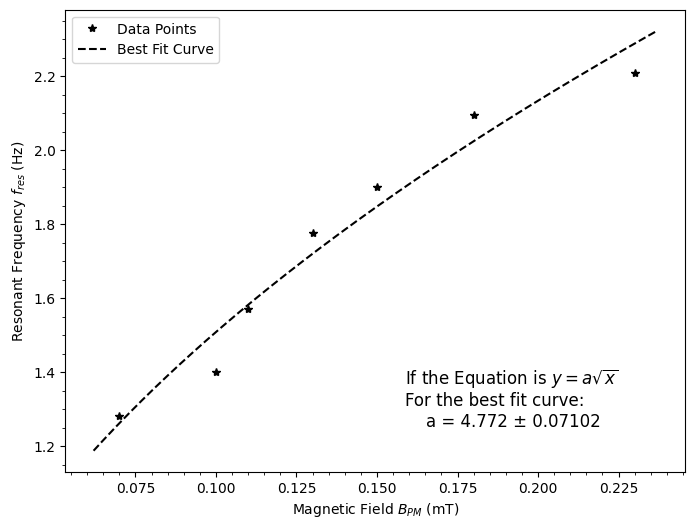
\includegraphics[width=1\columnwidth]{images/g.png}
    \caption{Plot of $f_\text{res}$ vs $B_{PM}$}
    \label{g}
\end{figure}